\documentclass{article}
\usepackage{graphicx}
\usepackage[margin=1in]{geometry}
\usepackage{comment}
\usepackage{titling}
\usepackage{textcomp}
\setlength{\droptitle}{-2.5cm}

\title{GPU Fault Tolerance}
\author{Toru Yamaguchi}
\date{}
\begin{document}
\maketitle
\vspace{-4em}
\section{Background}
The GPU was originally developed to handle graphics processing and multimedia, with its primary application in gaming and its main use in consumer desktops. Research around fault tolerance, which is the ability for a system to maintain its specified operations despite failure of one or more of its components, for GPUs wasn't seen as such a priority as it is today. Early research by NVIDIA~\cite{1} on the issue of transient faults (i.e. random, temporary defects) focused on faults that would only end up affecting the user's visual experience by a certain magnitude. The paper referenced the Architectural Vulnerability Factor (AVF)~\cite{1253181}, which is a strict metric to quantify whether a fault will progress to an architecturally visible error, and challenged it with the Visual Vulnerability Spectrum (VVS). This separate taxonomy for classifying transient faults on the GPU, aimed to relax fault tolerance in order to reduce unnecessary overhead, as most errors were deemed unnoticeable. Many pieces of literature in this area, including much of the papers cited here, like to mention in their introduction on how this unusually high tolerance to errors used to make up the view for GPU fault tolerance when it was first discussed. The gradual rise of General Purpose computing on GPU (GPGPU), instigated by incredible showcases of GPGPU performance~\cite{5446251}~\cite{4490127}, re-aligned the understanding towards GPU fault tolerance, from treating the non-graphical market as niche~\cite{2} to recognising it as an expansive area of critical research. GPUs have provided a new paradigm of performance for High Performance Computing (HPC), machine learning, and various safety critical applications, which has inevitably lead to an increased interest in supporting the reliability of these applications. In the following sections, after going through some terminology, we will review several key fault tolerance techniques for GPUs.

\section{Taxonomy and Basic Techniques}
GPUs are architecturally unique compared to CPUs, hosting thousands of cores designed to provide massive parallelism. Despite their differences, GPUs experience many of the same faults as CPUs. We will introduce the main taxonomy for hardware faults and their relevance to GPUs. Starting with permanent and intermittent faults, they describe faults caused by manufacturing defects and aging, with intermittent representing temporary versions of permanent faults. One study, GPBurn~\cite{6621133}, used extreme temperature tests to simulate accelerated aging, finding that at 170\textdegree C GPUs exhibit intermittent errors. As GPUs are continually adopted for automotive and space systems, where extreme temperatures are more frequent, this research helps to inform the state of GPUs to these faults. Further studies find some areas of the GPU, such as register files are naturally more robust towards permanent faults~\cite{6604089}. On the other hand, a more recent study~\cite{10.1145/3581784.3607086} found that parallelism management units (PMU) exhibit high levels (20\% to 60\%) of silent data corruption (SDC), which are errors that don't trigger alerts or crashes but produce incorrect results, and high levels of detected unrecoverable errors (DUE), which are errors that result in a crash or system hang, in Fetch/Decoder units ($>$90\%, 70\%). It's clear that several areas in the GPU are more prone to SDC/DUEs than others. The mention of SDCs and DUEs helps to expand our taxonomy to the class of transient faults, which were introduced earlier, and represent the bulk of fault tolerance research for GPUs. Early research showed that GPUs are not only susceptible to SDCs caused by transient faults~\cite{5493404} but as the device continues to shrink, the SDC rate will also rise~\cite{10.1145/1736020.1736063}. A hardware fault tolerance technique, error correcting codes (ECC), adds extra bits to memory data, which are checked when read to auto-correct single-bit errors and flag multi-bit errors. Whilst ECC significantly reduces the occurrence of SDCs, many papers find it insufficient by itself to consider GPUs as reliable~\cite{6962085}~\cite{7056044}~\cite{7975296}, nevertheless it is a fault tolerance technique that can be effective for applications that require it. Another technique, commonly found in CPUs brought to GPUs, is a checkpoint and recovery system (CPR), which creates periodic checkpoints during execution, resorting back to one in the event of a failure. Checkpointing the GPU status was introduced with CheCUDA~\cite{5372771}, and subsequently many iterations and improvements have been made as the GPU framework changes. Both ECC and CPR are essential techniques for fault tolerance, however, in the proceeding sections, we will dive deeper into other techniques that are crucial for GPU fault tolerance.

\section{Redundancy}
Redundancy is a common fault tolerance technique built on the premise that random faults are unlikely to occur at the same position for multiple instances of the same input. A good starting point would be a simple duplication of processes with comparison (DWC) for error detection, which unsurprisingly it sees double the execution time~\cite{10.1145/1513895.1513907}. Variations of DWC that duplicate instructions in either space or time~\cite{6949170} saw varied overheads 90\% to 151\% but found they reduced the SDC rate by one order of magnitude compared to ECC, mentioned previously. Several other techniques extend it by exploiting GPU hardware and software~\cite{6493606}~\cite{8665772}, such as utilising unused parallelism or by increasing the number of registers required for program execution, interestingly they find DWC has application dependent performance. This finding was supported by another redundancy technique called redundant multi-threading, involving one thread with full computation and another with minimal, which showed mixed performance~\cite{10.1145/2678373.2665686}. If the GPU optimisation involves utilising unused resources, which many redundancy optimisations do, this can explain the differing outcomes since certain applications may naturally use more resources than others. This insight into application dependent performance will be further explored later. If we turn our attention to safety-critical applications, the emerging use of GPUs demand high reliability. Triple mode redundancy (TMR) involves having three executions of a single process, with a voting system in place if we observe a fault in an execution. Implementations will try to avoid the expected 200\% overhead, such as Warped-RE~\cite{7266862} which exploits inherent redundancy between threads of the same warp. It uses dual mode redundancy (DMR) to detect errors but forces TMR if an error is detected, achieving an average overhead of just 29\%. However, this method will still suffer from additional overhead if the application has high resource utilisation. This re-occurring theme that the performance of redundancy is application dependent can bring forward the idea of selective redundancy. Explored in The Hauberk approach~\cite{6012845}, selective redundancy proposes that we observe and select the areas of the program with the highest error propagation for the most protection, thereby reducing unnecessary overhead. Many methods build on this approach, one used fault injections to examine vulnerable registers~\cite{8660708} and provided software/hardware based hardening such as register duplication to those areas. An important aspect of this method is choosing the critical areas (fault sites), this is often done through exhaustive fault injections (FI). However, research suggests that not all GPGPU fault sites are fault prone, with lots being considered redundant~\cite{8574583}~\cite{9035460}. This research is important when devising the FI process, with specific methodologies~\cite{9080079} being proposed to significantly reduce the FI campaign time. Redundancy has found its place as a staple method to effectively provide fault tolerance, as with most techniques, high reliability comes at the cost of performance, something safety-critical applications such as automotive systems have accepted~\cite{9523531}~\cite{9159153} to maintain reliability. This section has covered redundancy when applied to GPUs, with an emphasis on the lessons learnt, an important one being that many redundancy techniques find that performance is often application dependent, this is something at the very heart of our next fault tolerance technique.

\section{Algorithm Based Fault Tolerance}
\begin{figure}
    \centering
    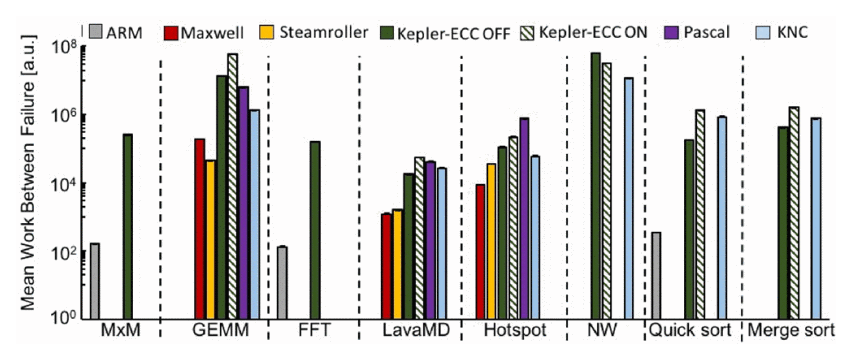
\includegraphics[width=0.8\textwidth]{pic.png}
    \caption{Injection results of different algorithms on CPUs and GPUs~\cite{8416467}}
    \label{Figure 1:}
\end{figure}
Algorithm Based Fault tolerance offers a different approach to reliability, like the name suggests, it implements hardening techniques to specific algorithms so that faults are detected based on the algorithm's result. The main method involves encoding the input data for the algorithm, modifying the algorithm to operate on encoded data, and finally to perform checks using checksums to validate the result. An insight into why ABFT has potential to work is given in figure~\ref{Figure 1:}, which shows the mean work between failure (MWBF) for several algorithms on different CPUs and GPUs. If we focus on Maxwell, Steamroller, Kepler, and Pascal as the GPU results, our main takeaway is that algorithms naturally exhibit different levels of failure, something ABFT is designed to consider. When it was first proposed~\cite{3}, ABFT pre-emptively highlighted its complementary nature with multi-processor systems, making it ideal for GPUs. A comparison of ABFT specifically with matrix multiplications (MM)~\cite{6604090} with techniques discussed previously such as DWC or TMR, highlighted the efficiency of ABFT, with added benefits such as avoiding unnecessary round-off error corrections, which is something ABFT with MM has seen strong results with~\cite{6903601}. Being the first algorithm to have ABFT applied to it, MM has seen various implementations on the GPU. A popular use case would be for Neural Networks, where reliable and efficient MM is required. Several studies\cite{8536419} show that ABFT outperforms other FT methods such as ECC, in detecting and correcting errors. A notable implementation~\cite{5951924} which moved the original method from off-line, meaning core computation and error checking are decoupled, to an on-line approach, where error checking is done during computation, provided the mechanism to immediately check for errors whilst being able to handle multiple errors. This approach has been used for various other studies such as combining it with kernel fusion~\cite{10.1145/3577193.3593715}, Cholesky Decomposition~\cite{7516096}, and Fast Fourier Transform~\cite{10.1145/3710848.3710853} making it a technique that can generalise to many algorithms. Conversely, an insight in ~\cite{7877099} suggests that more than 50\% of errors are masked within a single kernel execution, therefore checking for errors during computation as with on-line ABFT could produce unnecessary overhead. Its well known that the limitation to ABFT is its algorithm dependent nature, despite being the reason it has such a low overhead compared to techniques like TMR and DWC~\cite{6604090}. It can be seen though that GPU implemented algorithms aren't in abundance compared to CPU-based, due to its parallel constraints, most relying on efficient matrix and vector operations or linear algebra methods. This naturally allows most algorithms on the GPU to share properties that can be exploited further, something ABFT has managed to do to be a key fault tolerance technique for GPU applications.

\section{Conclusion}
We have reviewed various fault tolerance techniques for GPUs. Although GPUs are still primarily used for graphical applications, hence some hardware features such as ECC aren't enabled by default, the adoption of GPUs for HPC and safety-critical applications requires continued fault tolerance research especially as GPUs evolve for new use cases. As we look at the current state of GPUs, performance is still improving, but a study shows that continued reduction in execution times will not necessarily require more hardware and software sacrifices to maintain reliability~\cite{conclusion}, this is a positive sign for the future of GPU reliability.

\begin{comment}
Theres the argument that GPU fault tolerance is not as required, due to graphical applications like gaming still being the economic driving force behind GPU development, however the rise of gpu based machine learning, hpc etc is not something that can share relaxed fault tolerance. as chips get smaller and machine learning blah develops, the importance and rigour of gpu fault tolerance is something that will prove...
gpu devices for safety-critical...
mention GPU having different frameworks for reliability?
https://doi.org/10.1109/ISPASS.2016.7482077
https://doi.org/10.1016/j.parco.2013.01.001
https://doi.org/10.1109/CLUSTER59578.2024.00008 - tmr still exhibits SDC
https://doi.org/10.1007/s11227-024-06119-4 - increasing reliability doesn't have to decrease performance necessarily
conclusi
- abft, redundancy, can require more customised ways for error detection. is a generalised error detection not feasible?
- gpus are being used for less error tolerant applications, like ml, scientific computing, real-time, safety critical
    - "survey for safety critical" 
- inherently, adding more instructions and operations and checks to code, is akin to increasing the available code and execution that could be affected by faults
- "characterising accuracy aware.." argues that strict guarantees are often not reqired
real
- need more hardware based fault tolerance. leads to undesirable loss in performance. 


"A large-scale study of soft-errors on gpus in the field" 2016

"silent data corruptions at scale" 2021

"A methodology for comparing the reliability of gpu-based and cpu-based HPCs"


"Hard data on soft errors: A large scale assessment of real-world error rates in GPGPUs
- parity or ECC to memory subsystem would prevent memory-induced silent errors. 
\end{comment}


\bibliographystyle{unsrt}
\bibliography{references}

\end{document}
